\section{Semantic Triples Knowledge Graph}  \label{Knowledge_graph}

Modelling events as a set of semantic triples is a well-established technique in the field of news summarisation. There can be different rules for extracting entities and relations from the text (in this case, news articles) which result in the extraction of different types of relationships. These form a minimal representation of the corpus, are generally of type subject $subject \rightarrow predicate \rightarrow object$ and are called SPO triples.

In order to generate this triples, the text corpus can be segmented into and sentences and using the grammatical structure of the sentence, the subject, predicate and object can be extracted~\cite{retrospective_kg}~\cite{world2014rdf}.

An example of the SPO triple extracted from the sentence ``Elon Musk is the CEO of Tesla'' is `Elon Musk' (as subject), `CEO of' (as predicate) and `Tesla' (as object).

\begin{figure}[H]
    \centering
    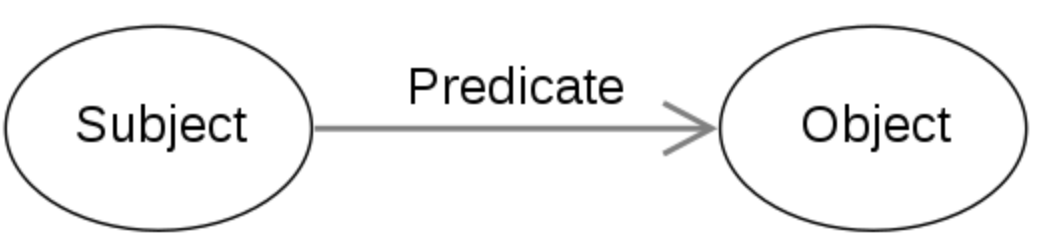
\includegraphics[width=0.3\textwidth]{images/spo.png}
\end{figure}

These triples are usually presented using a \textbf{Knowledge Graph}. A Knowledge Graph is a semantic graph which consists of nodes (vertices) and directed edges. The `subjects' and `objects' are represented as nodes and are usually entities and/or concepts. An entity can include a real-world physical object, for instance, a location (e.g. London), person (e.g. Paul McCartney), or an organization (e.g. WHO). Concepts, on the other hand, essentially refers to the general categories (that entities can belong to) such as airlines, websites, etc.~\cite{retrospective_kg}.

The `predicates' are represented as (directed) edges in a knowledge graph and are representative of the semantic relationships between entities and/or concepts derived by the descriptions of entities which have formal semantics. These descriptions usually highlight the key information about an entity and are interlinked (i.e., the description of one entity contributes to another) thereby resulting in the formation a graph~\cite{retrospective_kg} as shown in~\Cref{example_kg}.

\begin{figure}[H]
    \centering
    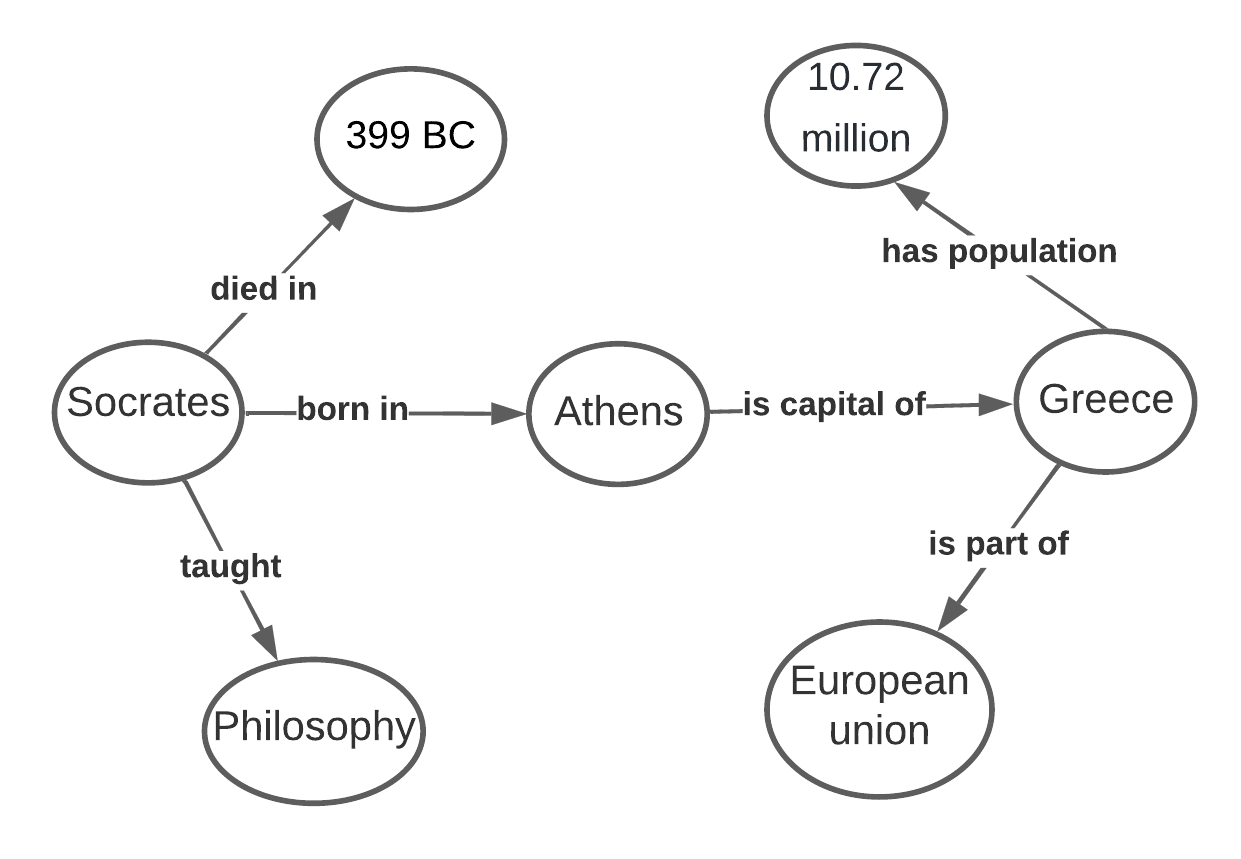
\includegraphics[width=0.6\textwidth]{images/eg_kg.png}
    \caption{An example knowledge graph}
    \label{example_kg}
\end{figure}

\subsubsection{Triple Store}

Given their particular, consistent structure, a collection of triples is often stored in purpose-built databases called Triplestores. A set of these triples represent an RDF graph, where the constituent of the triple (RDF term) can be of three types: ``internationalized resource identifier (IRI)~\cite{internationalized}, literal and blank nodes''. The ``subject can be an IRI or blank node, the predicate must be an IRI and lastly, an object can be an IRI, a literal or a blank node.''~\cite{6_world2014rdf}(p. 66). The RDF store complies with  W3C RDF and SPARQL standards. This is extremely useful as generally RDF triple stores use a query API SPARQL which enables the retrieval of relevant information~\cite{8_berven2020knowledge}.

\subsubsection{Ontology}

Ontology is a form of semantic knowledge representation. They can be used as a framework to build/ augment a knowledge graph. They model generalised types of objects (concepts, e.g. person), not the specific entities (e.g. Obama)~\cite{4_towards_kg}.

An ontology consists of: distinct types of objects called classes, the properties/ attributes of these classes as well as the relationships between the classes (directed edges). E.g., The class `Person' has a property `has\_DoB' and there is a relationship (directed edge) labelled `has\_DoB' from `Person' to the class `Date'~\cite{4_towards_kg}.

Two extremely common frameworks to model ontology are Resource Description Framework (RDF) and Web Ontology Language (OWL). They are standard frameworks thereby allowing easy exchange/ migration of data~\cite{4_towards_kg}~\cite{retrospective_kg}.


\subsubsection{Why are knowledge graphs useful? }

Knowledge graphs construction can be particularly useful as: 

\begin{itemize}
\item They are able to extract information from semi-structured, structured, and/or unstructured data sources, combining knowledge to a well-represented graph structure~\cite{retrospective_kg}. 

\item They incorporate the functionality of multiple storage types. For example, like databases, queries can be used for data retrieval and like knowledge bases, data stored has formal semantics, which can be used to interpret and infer data~\cite{2_guide_kg}. 

\item They can perform logical reasoning/ inference by exploiting graph structure. For instance, by traversing the graph, it can be inferred that C is grandmother of A if B is mother of A and C is mother of B (transitive relations)~\cite{2_guide_kg}. 
\end{itemize}  


\subsubsection{Examples of Big Knowledge Graphs}

\begin{itemize}
\item Google knowledge graph (GKG):  Google uses GKG to incorporate semantic search functionality into its search engine for topic inference from the search query. It contains over ``3.5
billion facts over 500 million objects/ entities''~\cite{retrospective_kg}(p.68)

\item DBPedia: is a crowd-sourced, multilingual knowledge base (RDF) which uses Wikipedia to extract structured data. It has approximately "24.9 million things in 119 languages, with 4.0 million things in English"~\cite{retrospective_kg}(p.68).

\item Wikidata: is a free, multilingual, crowd-sourced
knowledge base, It contains structured data and supports Wikimedia projects. Wikidata has more "than 59 million entities". It has a powerful SPARQL query interface allowing for ad-hoc visualisations~\cite{ieee_named_entity}. 

\end{itemize}

% ---------------------------------------------------------------------------------------------------------


\section{Principals of Visualisation} \label{principal_vis}

For the scope of the project, there needs to be some visualisation tool to display the results of semantic analysis of news. Therefore, in this section, we look at the important considerations to build  coherent, effective visualisations. 

First and foremost, it is important to understand the goal of the visualisation, what precisely is needed to be visualised and think about what type of data is required for this. This data (in this case, news articles) can then be processed to transform and summarise it, extracting key pieces of information that is determined to be essential to the application. This transformed data can then be stored in our desired format and utilised to output the visualisation.

The following highlight the key principles of visualisation:

\begin{enumerate}
\item \textbf{Simple:}
It is important to ensure that the visuals are simple and intuitive. The information that is most relevant to the application must be clearly and succinctly visible and organised in a consistent manner. Adding any unnecessary information can make the visualisation convoluted and difficult to understand~\cite{29_bhalla_2022}. 

\item \textbf{Standard:}
Standardisation of data structure and elements is needed for a good visualisation. This requires handling any complexities and discrepancies in the data as well as eliminating redundancies. Examples of this include, but are not limited to, using common abbreviations, identical scaling, consistent layouts across your data visualisations~\cite{29_bhalla_2022}. Additionally, it is important to provide context for these visualisations as well by using standardised labelling and indexing~\cite{30_vis}.

\item \textbf{Scalable:}
Scalability, in this context, refers to the ability of a visualisation to adjust with the increasing volumes of data seamlessly. This increase should have minimal impact on the speed as well as the performance of the program. Additionally, this also relates how to fit the virtualisation by dynamically scaling it to the virtual space as it grows~\cite{29_bhalla_2022}. 

\item \textbf{Identify target audience:}
 For the visualisation to be a good representation of the data, it is important to identify the target audience and how they will interact/ use the visual. As mentioned before, exploiting visual details like size, colour, position, font etc can allow for a more intuitive design whilst directing the focus of the users to key bits of information\cite{30_vis}. 

\item \textbf{Making use of interactivity:}
It can be useful to leverage the interactivity in the visualisation, thereby allowing for a multi-faceted visualisation based on the context that the users choose. For example, if a user wants to the see key news related to the airline industry, the visualisation can zoom in to focus on the part of the visualisation specific to that sector. User interactions should be intuitive and simple to not confuse the user and discourage participation. 

\end{enumerate}


% \subsection{Future work: Self-Organising Maps}

% Self-organising maps (SOM), also known as Kohonen maps, is a type of neural network that uses unsupervised learning and aims to reduce continuous high multidimensional data onto discrete low dimensional by making use of a feature map and neighboured function based on some metric of similarity. They make use of topographic maps which follow the "principle of topographic map formation" where each new piece of information will be stored in its neighboured (derived from context). Additionally, neurons accessing related information will be stored nearby for quick interactions and updates. \hyperlink{26}{[26]} 

% The SOM algorithm consists of four key stages:\hyperlink{26}{[26]}\hyperlink{27}{[27]}

% \begin{enumerate}
%     \item \textbf{Initialization: }
%     This is where all the weights of neurons are initialised with small values that are randomly generated. 
    
%     \item \textbf{Competitive stage: }
%     In this stage, the algorithm picks the best matching or 'winning' neuron by computing a discriminant function. The competitive aspect arises from the fact that the neuron with the smallest value for this function is the 'winning' neuron. Euclidean distance is often picked as the discriminant function. Therefore, for an input vector v, the best matching neuron is the neuron whose weight is the smallest Euclidean distance away. This is generally referred to as Best Matching Unit (BMU). So, for neurons (n) and a randomly drawn input sample v, the BMU can be determined by: \hyperlink{27}{[27]}

%     \begin{center}
%          $ n_{BMU} = argmin_{n} \left\lVert w_{n} - v \right\rVert $
%     \end{center}


% \item Cooperative stage: 
%     This stage makes sure that the weights of the neurons in the same neighbourhood have an effect on each other and are not modified independently of one another. Once the winning neuron is established, the weight of this 'winning' neuron is updated. However, now similar updates to the weights of the neighbouring neurons must also be made. This requires a neighbourhood function that gets the topological neighbourhood of a neuron which is centred (symmetrical) around the winning neuron and decays with increasing (lateral) distance. This function $\Lambda$ can be defined as follows: 
%     \begin{center}
    
%         $\Lambda(i, j) = \frac{( \left\lVert r_{i} - r_{j} \right\rVert)^2}{2\sigma^2} $
        
%          \end{center}
         
%         where  i is the winning neuron and $\left\lVert r_{i} - r_{j} \right\rVert$ is the  lateral (lattice) distance of neuron j from the winning neuron and $\sigma$ is the standard deviation which decays exponentially with time. This is useful as this method is translation invariant. \hyperlink{26}{[26]}\hyperlink{27}{[27]}
        
        
% \item \textbf{Adaptive process: }
%         In order to get the features mapping the input space to the output space, a learning process is involved. This uses a learning parameter ($\alpha$) that decays over time (iterations/ epochs). From this, the weight rule can be defined as follows:
        
%         \begin{center}
    
%         $ w_{i} = \alpha (t) \Lambda (i, j, t) (v - w_{i})$
        
%          \end{center}
       
%       The weight updates will gradually move the winning neuron's (i) weight as well as its neighbouring neurons to be close to the input vector. The closer the neighbouring neuron j to the winning neuron, the greater the change to its weight. Over time/epochs, the radius of the neighbourhood decreases (so the number of neighbours decreases). This is done to promote the learning to have a significant effect on the weights (of neurons) during the initial/early iterations but not allow them to be  influenced by far away neurons in later stages of the training (encouraging convergence) \hyperlink{26}{[26]}
       
% \end{enumerate}

% \section{Summary of Research}
% To summarise the background research discussed in this chapter, 